\documentclass[a4paper]{scrartcl}

\usepackage{graphicx}
\usepackage{url}

%% Limit: 40000 chars
%% check with `detex paper.tex | wc -c`

\title{DNSKEY Management}
\author{Julien Perrochet \and Tobias Schlatter}
\date{December 12, 2012}

\graphicspath{{../figures/}}

\newcommand{\wbjp}{\protect\footnote{Written by Julien Perrochet}}
\newcommand{\wbts}{\protect\footnote{Written by Tobias Schlatter}}


\begin{document}

\maketitle

\section{Introduction}
%% TODO add some blah about management and penetration.

In the following, every necessary operation for key management in
DNSSEC is described as a reminder to the reader.

\paragraph{Enabling DNSSEC} When enabling DNSSEC for a zone, the
parent zone has to establish and sign a DS record with the newly
created public-key.

\paragraph{Key Rollover} RFC4641 \cite{RFC4641} suggests that the DNSKEY
records for a zone should be changed somewhere between once every week
up to once every month. While the detailed rollover procedure is
irrelevant here, it is important to know, that the parent zone has to
update the its DS record.

\paragraph{Disabling DNSSEC} An operator might choose to discontinue
DNSSEC for a zone. The DS records (or other means of signing DNSKEYs
as we will see later) need to be removed.

\section{DNSSEC Deployment\wbts}

This section shall expose the current deployment status of DNSSEC.

\subsection{Penetration}

In figure~\ref{fig:dnssec-growth} you can see the development of
deployed, production DNSSEC zones (for the heuristics applied to
determine a production zone, see \cite{secspider, Osterweil09}). We
can see that DNSSEC is gradually being deployed.

Contrary to the state at writing of \cite{Osterweil09}, the DNS
root-zone is signed since July 15, 2010 \cite{root-dnssec} and hence
serves as the global trust anchor. However, as of this writing,
data\footnote{\url{http://secspider.cs.ucla.edu/islands.html}}
gathered by \cite{secspider} suggests that more than half of the
deployed DNSSEC zones which are verifyable (i.e. are likely not to
have a spoofed key, see \cite{Osterweil09} for details), do not yet
have a fully linked certificate chain up to the root zone.

\begin{figure}
  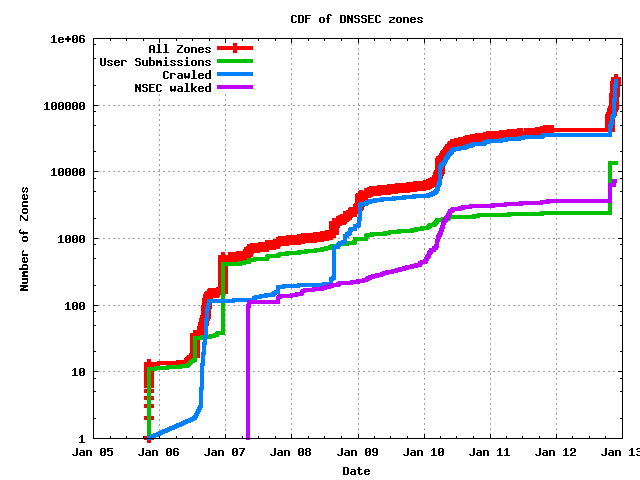
\includegraphics[width=\linewidth]{dnssec-growth}
  \caption{Number of deployed DNSSEC zones by
    SecSpider \cite{secspider}}
  \label{fig:dnssec-growth}
\end{figure}

\subsection{Trust Anchors}




\section{Operations\wbjp}
\subsection{3Rs}
\subsection{Single admin}
\subsection{Multi admin}
\subsection{Disabling}

\section{Case-Study: Switzerland (\texttt{ch.} Zone)\wbts}
According to a query on \cite{secspider}, the \verb|ch.| TLD zone is signed and
fully veryfiable from the root zone anchor. The validity period of a
zone signing key is 37 days \cite{switch10}.

\nocite{*}
\bibliographystyle{abbrv}
\bibliography{dnssec}

\end{document}

%%% Local Variables: 
%%% mode: latex
%%% TeX-master: t
%%% End: 
